\documentclass[aps,twocolumn,secnumarabic,balancelastpage,amsmath,amssymb,nofootinbib,floatfix]{revtex4-1}

\usepackage{graphicx}      % tools for importing graphics
\usepackage[colorlinks=true]{hyperref}  % this package should be added 
\usepackage{dcolumn}% Align table columns on decimal point
\usepackage{bm}% bold math
\usepackage{xcolor}

\newcommand{\ev}{\,{\rm eV}}
\newcommand{\nm}{\,{\rm nm}}
\newcommand{\pA}{\,{\rm pA}}


\begin{document}

\title{Photoelectric Effect}

\author{Vinh Tran}
\affiliation{Department of Physics and Kavli Institute for Astrophysics and Space Research, Massachusetts Institute of Technology, Cambridge, MA 02139, USA}
\email{vinhtran@mit.edu}

\date{\today}

%%%%%%%%%%%%%%%%%%%%%%%%%%%%%%%%%%%%%%%%%%%%%%%%%%%%%%%%%%%%%%%%%%

\begin{abstract}

\end{abstract}

\maketitle

%%%%%%%%%%%%%%%%%%%%%%%%%%%%%%%%%%%%%%%%%%%%%%%%%%%%%%%%%%%%%%%%%%

\section{Introduction}
\label{sec:intro}

The photoelectric effect, first discovered by Heinrich Hertz~\citep{1Hertz887} in 1887 and later explained by Albert Einstein~\cite{Einstein1905} in 1905, describes the process in which charge particles are released from the metal surface by light of short-enough wavelength $\lambda$. In his work, Einstein characterized light as quanta of energy $h \nu$, with $h$ as the Plank constant and $\nu = c/\lambda$ as the light wave frequency. These light particles (i.e. photons) deposit energy into the charge particles (typically electrons) and push them out of the metal surface, overcoming the potential well. The depth of these potential wells, called the work function $\phi$, can be calculated as the difference between the photon energy $h \nu$ and the ejected charge particle's kinetic energy $K$
\begin{equation}
    \label{eqn:work_function}
    h \nu = K + \phi.
\end{equation}
A more general summary of the photoelectric effect can be found in the review by Klassen~\citep{Klassen2011}.

In this experiment, we perform a measurement of the Plank constant $h$ through the identification of the work function $\phi$ and the cut off voltages, i.e. the voltages at which the photoelectric current is zero, for different wavelengths. In Section~\ref{sec:experiment}, we describe the experimental apparatus and the data collection process. In Section~\ref{sec:result}, we present the results of the experiment and discuss the implications of the measurements. Finally, in Section~\ref{sec:conclusion}, we summarize the findings and provide a conclusion.


\section{Experiment Setup}
\label{sec:experiment}

\subsection{Apparatus}
\label{sec:apparatus}

\begin{figure}
    \centering
    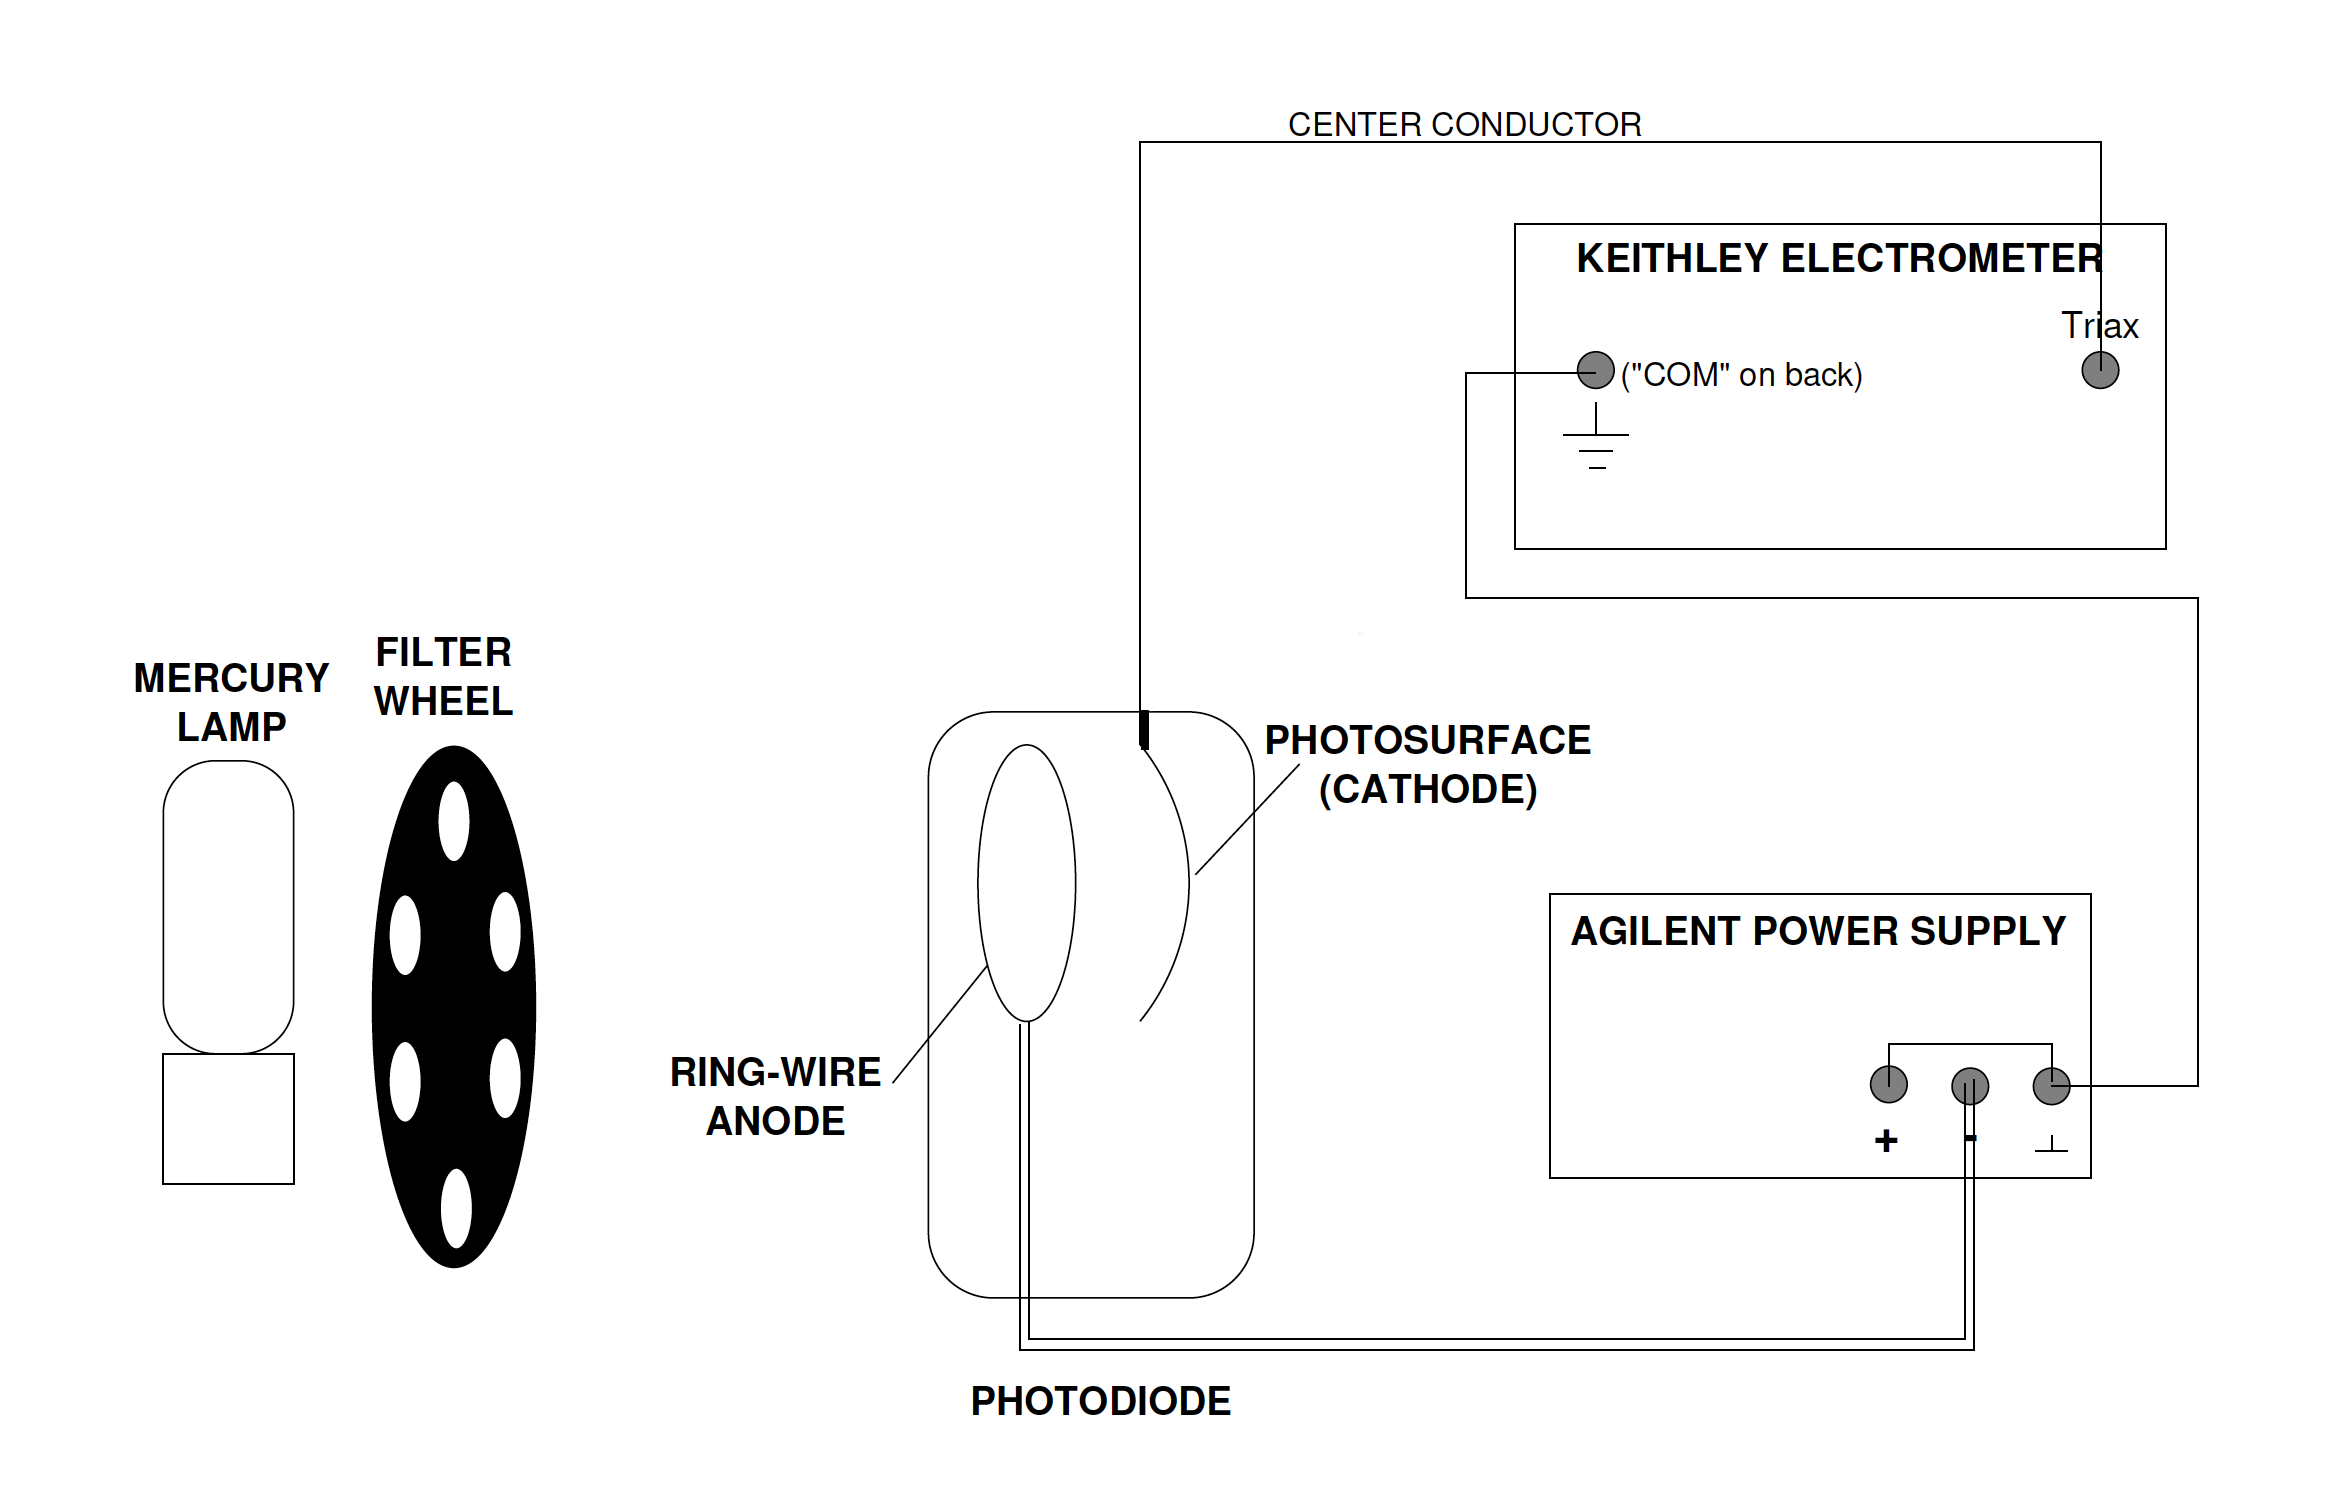
\includegraphics[width=0.49 \textwidth]{Figures/apparatus.png}
    \caption{The experiment apparatus, reconstructed from~\citep{MITPhotoelectricEffect}.}
    \label{fig:apparatus}
\end{figure}

The experiment utilizes the photoelectric apparatus shown in Figure~\ref{fig:apparatus}, following~\citep{MITPhotoelectricEffect}, which consists of a mercury lamp, a filter wheel, a photodiode, which comprises of a potassium photosuface (cathode) and a platinum-rhodium alloy ring wire (anode) with significanly higher work function compared to the photosurface, a voltage supply, and a Keithley electrometer. The positive terminal of the power supply is connected to the ground terminal and to the cathode of the photodiode (with the Keithley electrometer connected inbetween), while the power supply's negative terminal is connected to the photodiode's anode. This create a reverse (retarded) voltage $V$ across the photodiode, which can be adjusted to control the photoelectric current. The mercury lamp emits sharp emission peaks at different wavelengths, which can be selected by the filter wheel. We perform measurements for the wavelengths of $\lambda = 365.0, \, 404.7, \, 435.8,$ and $546.1\nm$, with the bandwidth of the filters of the order of $4.0\nm$. Light is then directed to the photosurface of the photodiode's cathode, where a current $I$ is generated for photons of sufficient energy, i.e. enough to overcome the work function $\phi$ and the retarded voltage $V$. The current is then measured by the Keithley electrometer. We pay special attention to the grounding of equipment and the alignment of apparatus to ensure the accuracy of the measurements.

\subsection{Data Collection}
\label{sec:data_collection}

As demonstarted by various experiments~\citep[e.g.][]{Millikan1916,Quinn1964,Wong2011}, the voltage boundary manifests not as a clear cut off, but rather as a gradual reduce in currect, approaching an asymptotic flat regime. Additionally, as the retarded voltage further increase, the phenomenon of reverse current, where photoelectons emitted from light hitting the anode travel toward the cathode, occurs. Adapting our data collection stratergy according to these phenomenon, we measure the photoelectric current across a wide range of retarded voltages using semi-uniform steps. 

The current $I$ is typically of the order of $10 \text{--} 100\pA$, so further precautions in the apparatus arangement, e.g. the arangement and length of connecting wires, are required. At these scales, the fluctuation of the current also appear to be of important. Therefore, at each volatge, we record the different values of $I$ and obtain the central value $\mu_I$ and standard deviation $\sigma_I$ following the Bayesian principle with equal probability priors $p(\boldsymbol{\theta})$, where $\boldsymbol{\theta} = (\mu_I,\sigma_I)$, and the maximum a piori cost $C_{\rm{MAP}} (\boldsymbol{\theta} - \boldsymbol{\theta^\prime}) = \delta (\boldsymbol{\theta} - \boldsymbol{\theta^\prime})$. The values of $\mu_I$ and $\sigma_I$ follow
\begin{equation}
    \label{eqn:I_bayesian}
    \mu_I,\sigma_I =  \arg \min_{\mu_I,\sigma_I} - 2 \log{\mathcal{L} (\mu_I,\sigma_I)},
\end{equation}
where
\begin{equation}
    \label{eqn:I_NLL}
    - 2 \log{\mathcal{L} (\mu_I,\sigma_I)} = N \log{2 \pi \sigma_I^2} + \sum_i \left(\frac{I_i - \mu_I}{\sigma_I}\right)^2
\end{equation}
is the negative log likelihood function, $N$ is the number of measurements, and $I_i$ is the current at the $i$-th measurement. Onward, we denote $\mu_I$ as $I$ for simplicity. The approach performs well as the residual sum of squares $RSS = \sum_i (I_i - I)^2 / \sigma_I^2$ exhibit the typical expected value of the $\chi^2$ distribution of $N$ degrees of freedom.

To isolate the photoelectric effect from the background signal and other voltage-dependent effects, we also measure the currents at the same voltages but with the light source blocked. The background current $I_{\rm{bg}}$ is then subtracted from the total current $I_{\rm{total}}$ to obtain the photoelectric current $I_{\rm{pe}} = I_{\rm{total}} - I_{\rm{bg}}$.

\section{Results}
\label{sec:result}

\begin{figure}
    \centering
    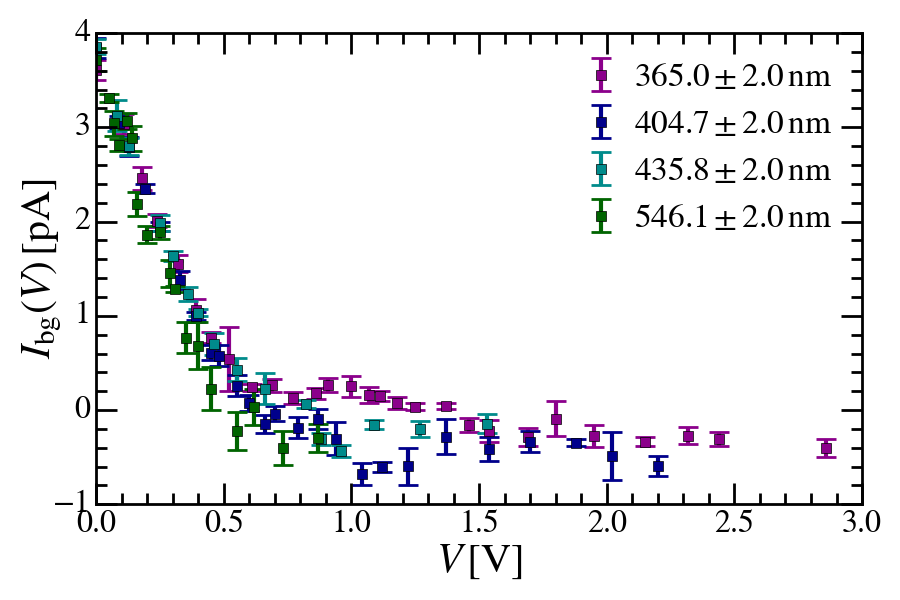
\includegraphics[width=0.49 \textwidth]{Figures/background.png}
    \caption{}
    \label{fig:background}
\end{figure}

\begin{figure}
    \centering
    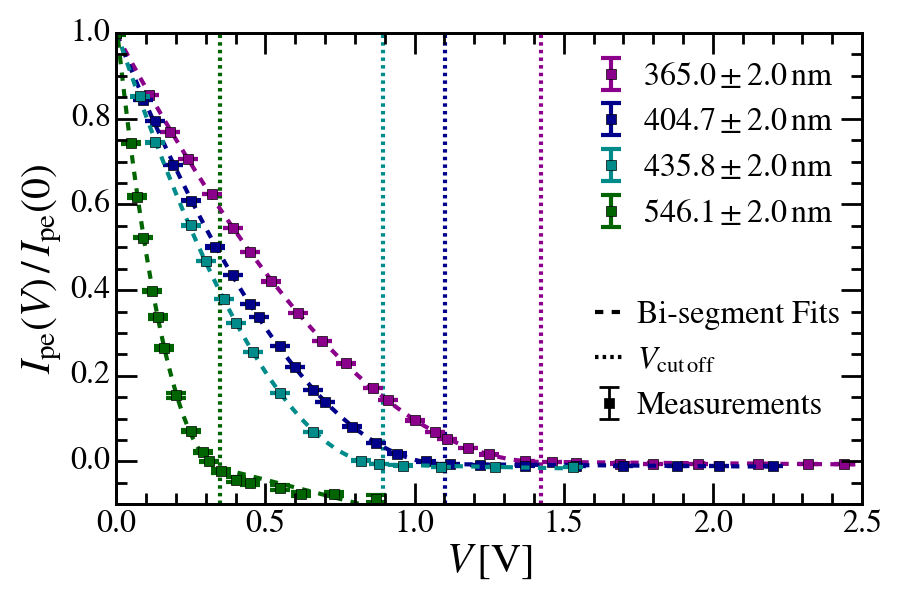
\includegraphics[width=0.49 \textwidth]{Figures/measurements.png}
    \caption{}
    \label{fig:measurements}
\end{figure}

\begin{figure}
    \centering
    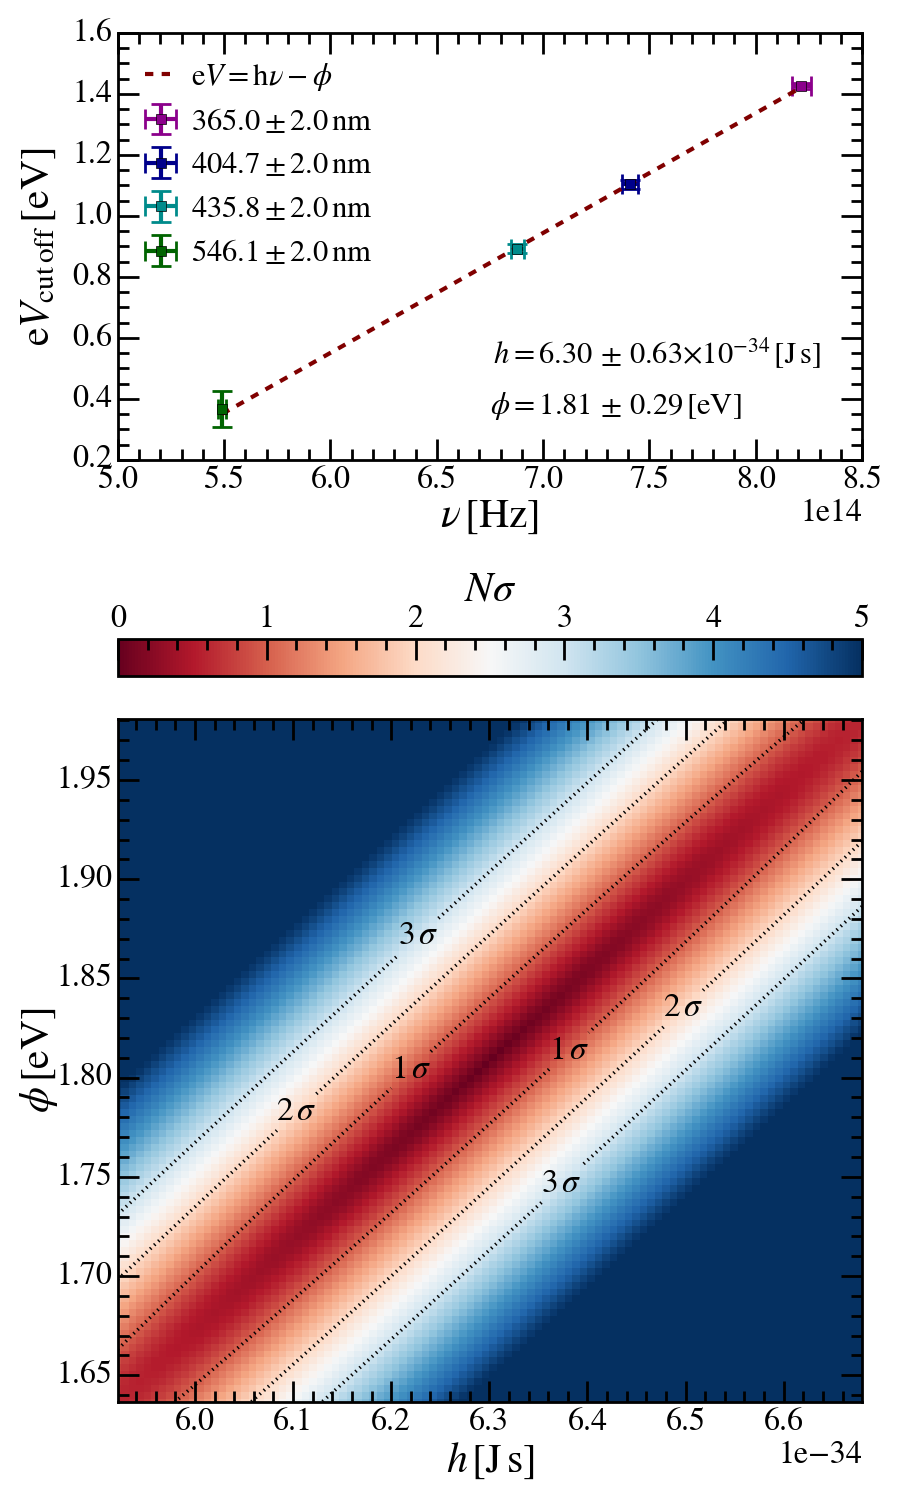
\includegraphics[width=0.49 \textwidth]{Figures/plank_and_work_function_fit.png}
    \caption{}
    \label{fig:h_and_phi}
\end{figure}

\section{Discussion and Conclusion}
\label{sec:conclusion}

%%%%%%%%%%%%%%%%%%%%%%%%%%%%%%%%%%%%%%%%%%%%%%%%%%%%%%%%%%%%%%%%%%

\bibliography{main}

%%%%%%%%%%%%%%%%%%%%%%%%%%%%%%%%%%%%%%%%%%%%%%%%%%%%%%%%%%%%%%%%%%

\appendix

\section{Monte Carlo Sample Fits}

\begin{figure}
    \centering
    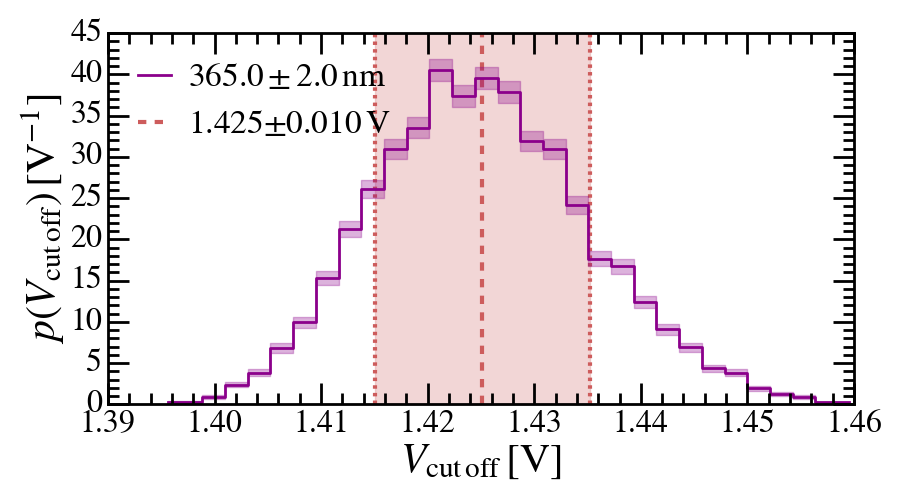
\includegraphics[width=0.49 \textwidth]{Figures/V_cutoff_365nm.png}
    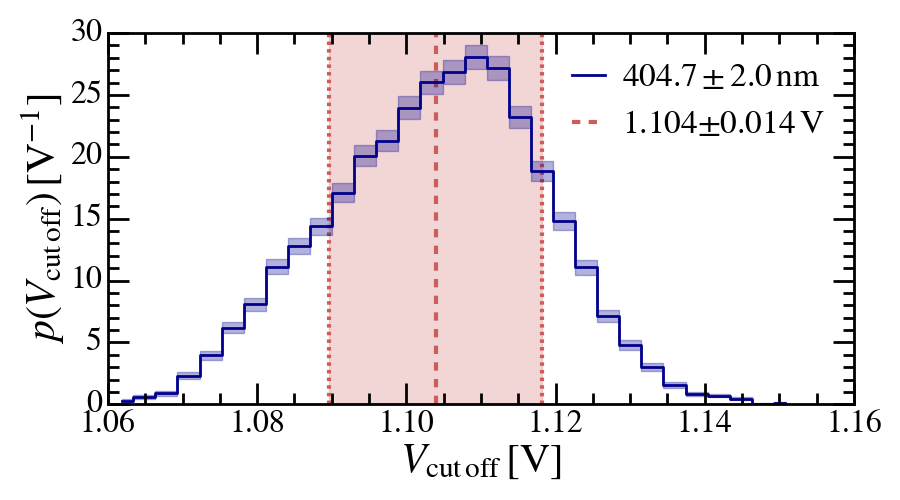
\includegraphics[width=0.49 \textwidth]{Figures/V_cutoff_405nm.png}
    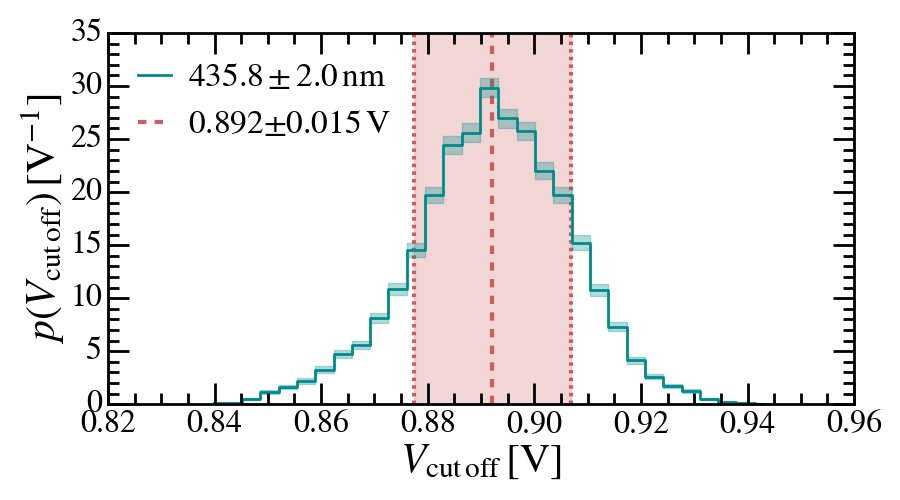
\includegraphics[width=0.49 \textwidth]{Figures/V_cutoff_436nm.png}
    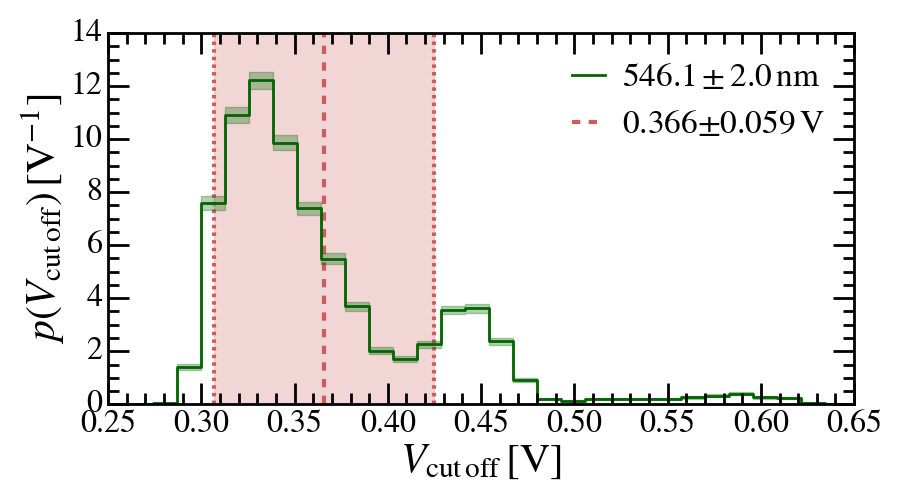
\includegraphics[width=0.49 \textwidth]{Figures/V_cutoff_546nm.png}
    \caption{The results of 10000 Monte Carlo sample fits for the cut off voltage at different wavelengths, following the procedual described in Section~\ref{sec:result}. The histograms show the distribution of the cut off voltage $V_{\rm{cut\,off}}$, while the dashed red line and shaded regions represent the central fitted values and their standard deviations. For the three shorter wavelengths, the fits are generally well behaved, with a unimodal Gaussian-like distribution. On the other hand, the longest wavelength of $546.1\nm$ shows a bimodal distribution, which may be the result of the limited measurements.}
    \label{fig:MC_fitting}
\end{figure}

\end{document}